\chapter{Aplicação exemplar}\label{chapter-aplicacao}

\chapterprecis{Este capítulo apresenta a aplicação exemplar desenvolvida.}\index{sinopse de capítulo}

O código fonte está disponível no repositório do GitHub com link \url{https://github.com/Jp9910/microservices_project}

% \section{Domínio}
A aplicação desenvolvida trata-se de um sistema web de e-commerce. Nela, um cliente da loja pode buscar e comprar produtos, enquanto um administrador pode gerenciar produtos e usuários cadastrados, tudo a partir de uma interface de usuário em um navegador.

Os diagramas de classes, pacotes e componentes podem ser vistos na \autoref{figura-diagrama-de-classes}, \autoref{figura-diagrama-de-pacotes} e \autoref{figura-diagrama-de-componentes}, respectivamente.

\section{Divisão dos microsserviços}
% TODO: diagramas de classes, de pacotes, e de sequencia dos microsserviços

\subsection*{Serviço de negócios - Loja}
Esse microsserviço trata da lógica de negócios relacionada a produtos e pedidos.

\subsection*{Serviço de negócios - Carrinho}
Esse microsserviço trata da lógica de negócios relacionada ao carrinho e realização da compra.

\subsection*{Serviço de negócios - Usuários}
Esse microsserviço trata da lógica de negócios relacionada ao cadastro e autenticação de usuários.

\subsection*{Serviço de negócios - Financeiro}
Esse microsserviço trata apenas do processamento (fictício) do pagamento de um pedido.

\subsection*{Serviço de ponta - Clientes}
O microsserviço de ponta de clientes é o serviço acessado diretamente pelos clientes da loja para realizar todas as operações relevantes a eles a partir de uma interface de usuário, tal como ver e buscar produtos, adicionar produtos ao carrinho e realizar um pedido a partir de um carrinho.

\subsection*{Serviço de ponta - Administração}
O microsserviço de ponta de administração é o serviço usado pelos administradores da loja para realizar todas as operações relevantes a eles a partir de uma interface de usuário, tal como gerenciar produtos e usuários.


\begin{figure}[htb]
	\caption{\label{figura-diagrama-de-classes}Diagrama de classes da aplicação exemplar}
	\begin{center}
	    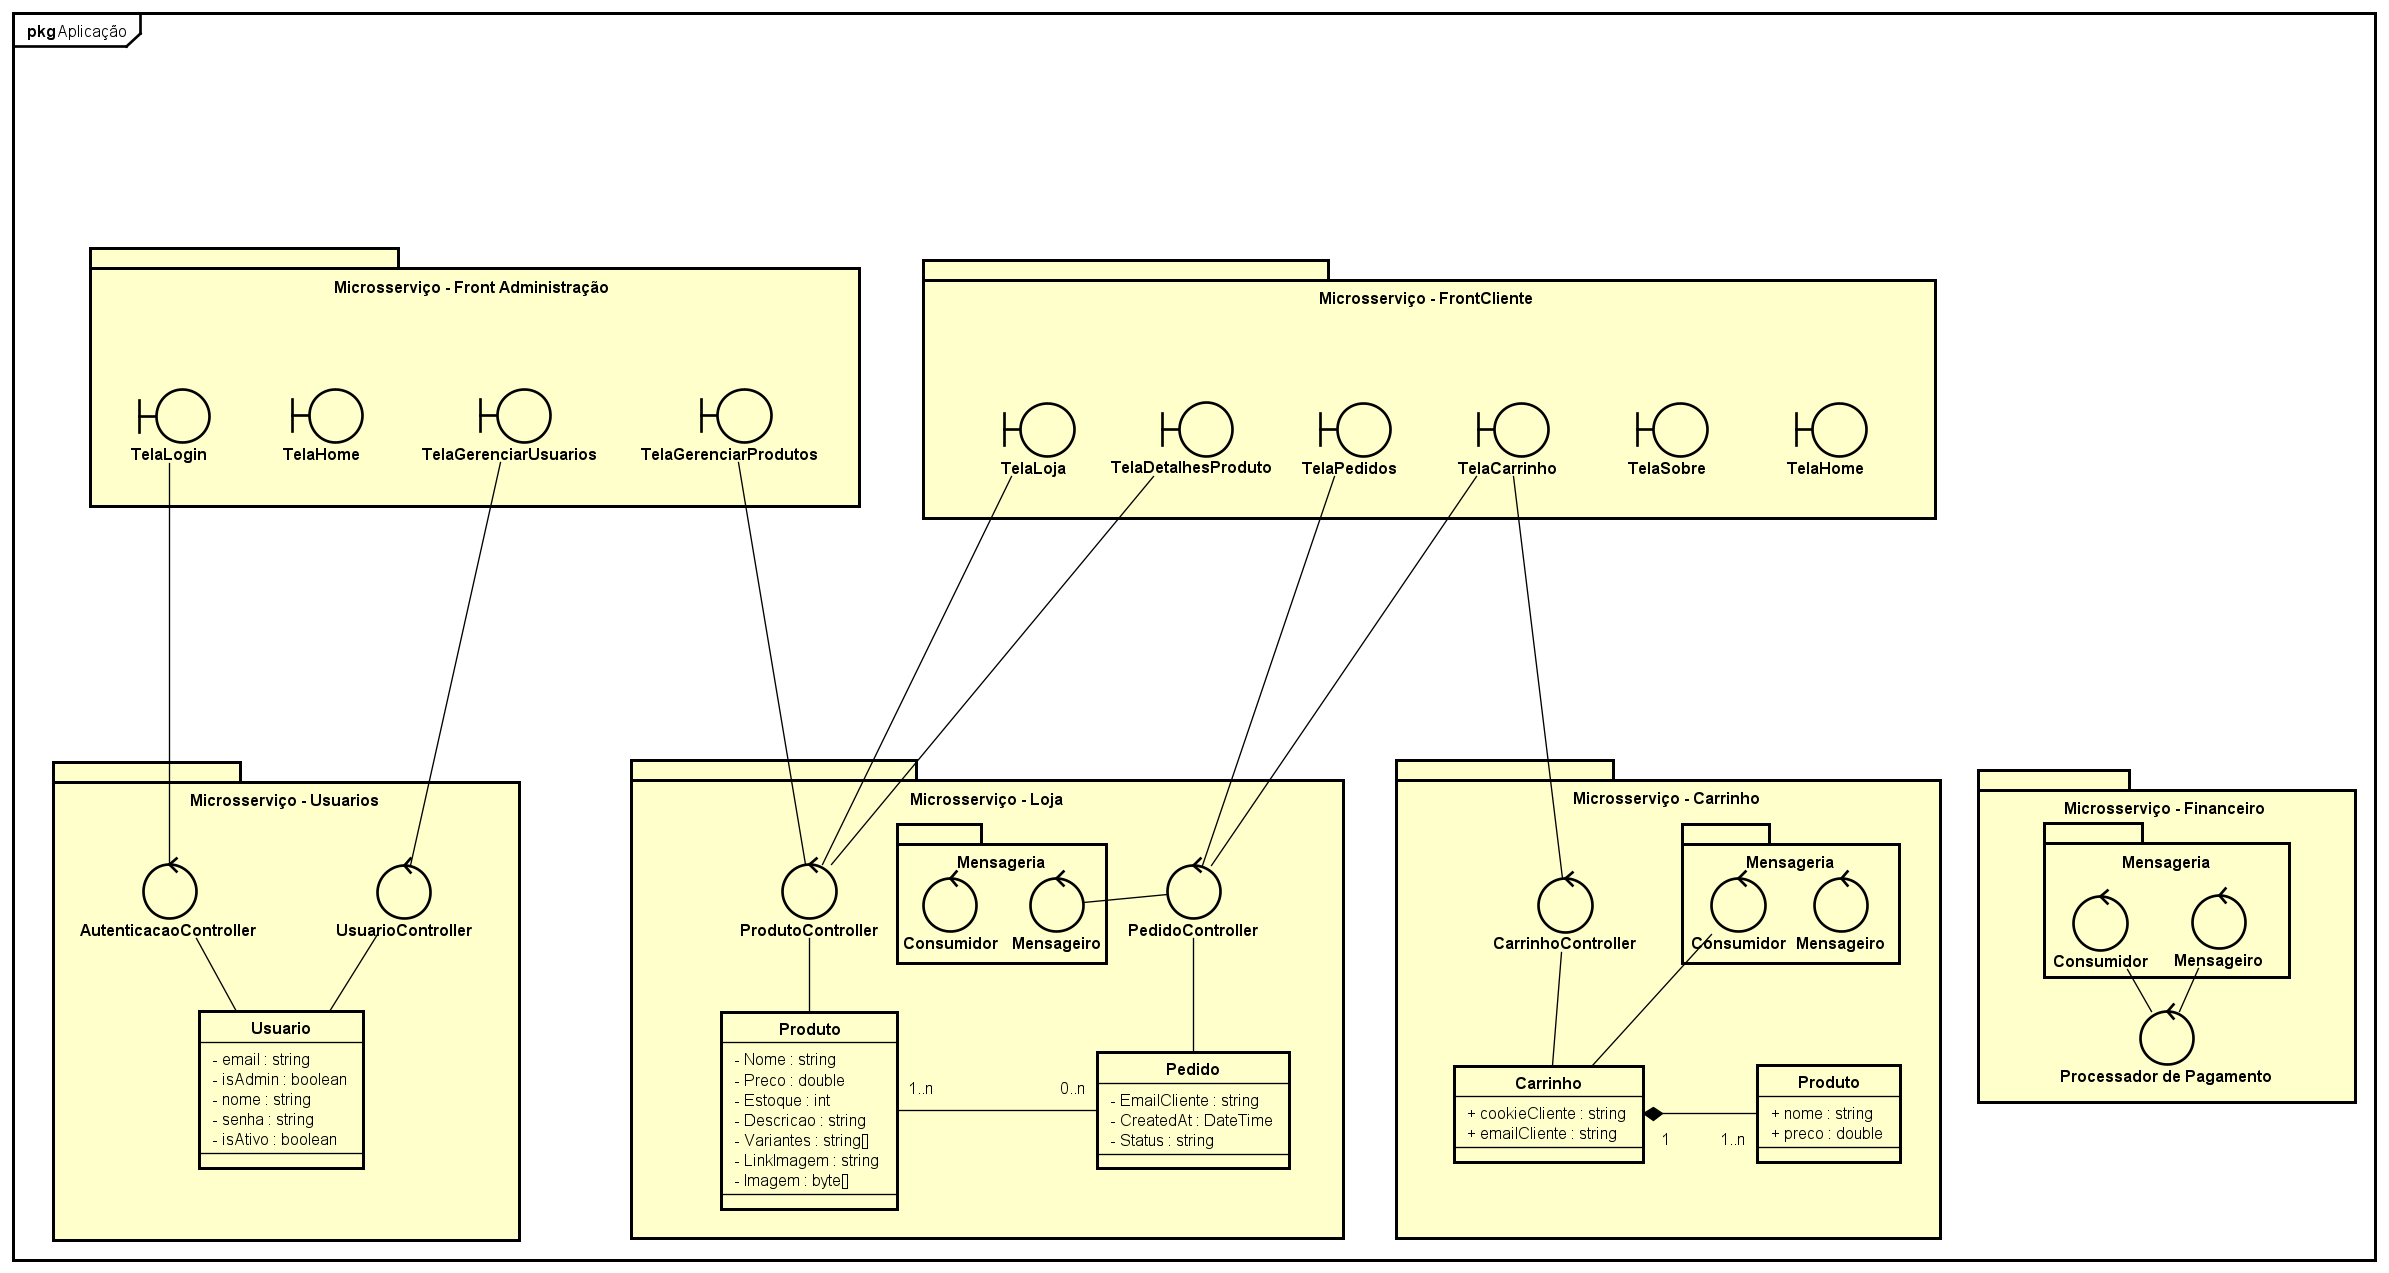
\includegraphics[scale=0.25]{Diagramas/imagens/ClassesComFinanceiro.png}
	\end{center}
	\legend{Fonte: Autor}
\end{figure}

\begin{figure}[htb]
	\caption{\label{figura-diagrama-de-pacotes}Diagrama de pacotes da aplicação exemplar}
	\begin{center}
	    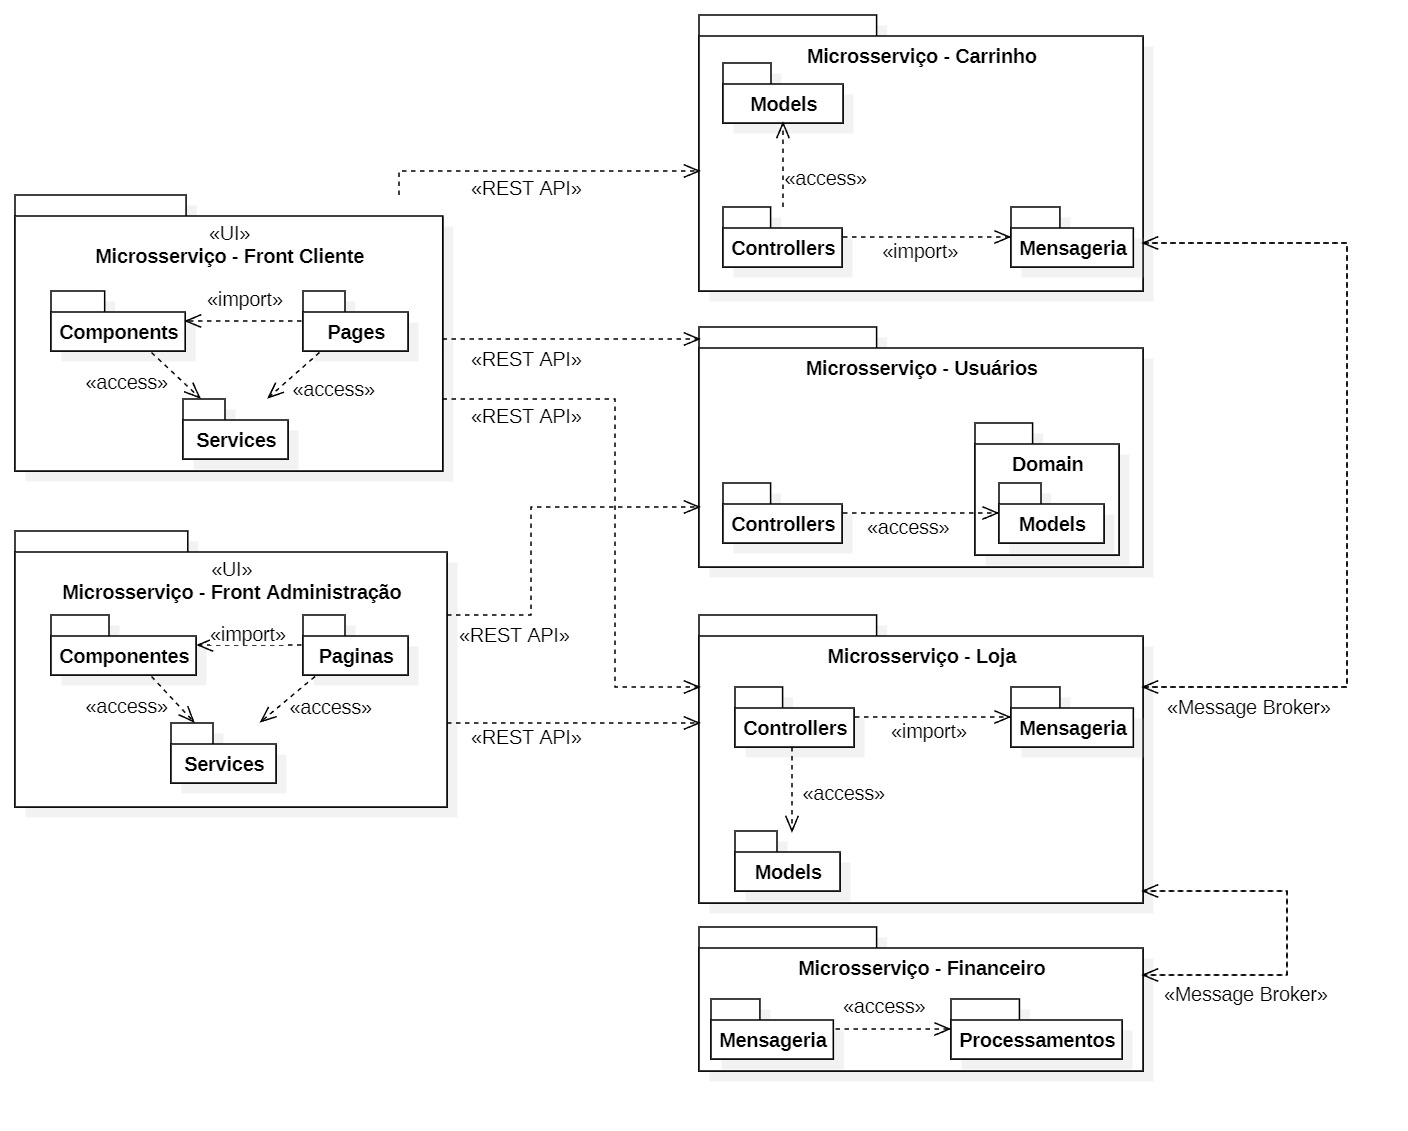
\includegraphics[scale=0.27]{Diagramas/imagens/PackageDiagramComFinanceiro.jpg}
	\end{center}
	\legend{Fonte: Autor}
\end{figure}

\begin{figure}[htb]
	\caption{\label{figura-diagrama-de-componentes}Diagrama de componentes da aplicação exemplar}
	\begin{center}
	    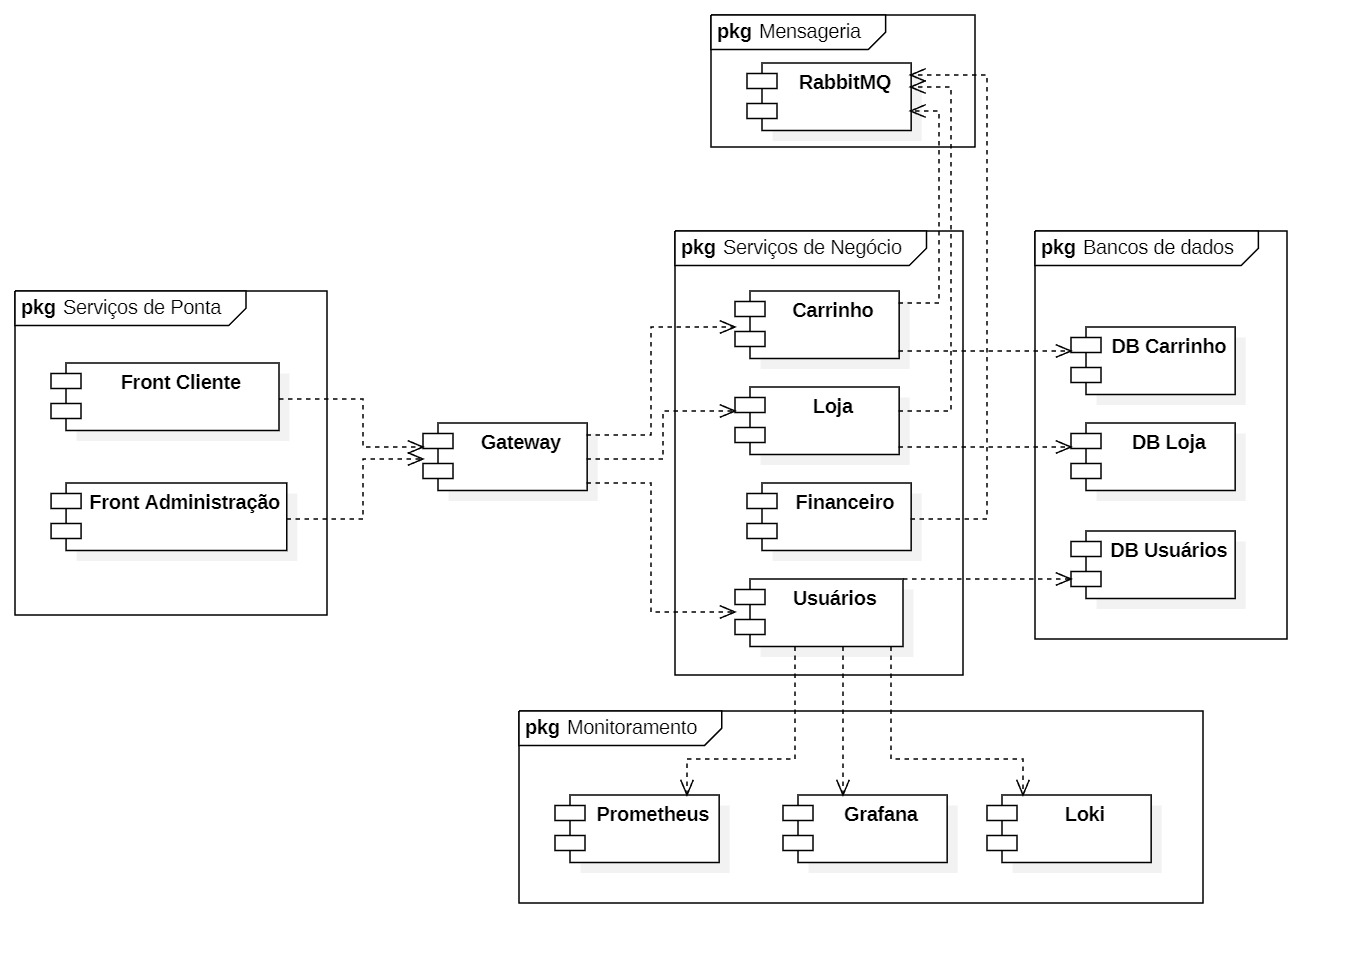
\includegraphics[scale=0.27]{Diagramas/imagens/ComponentsComFinanceiro.jpg}
	\end{center}
	\legend{Fonte: Autor}
\end{figure}

\begin{figure}[htb]
	\caption{\label{figura-diagrama-de-sequencia}Diagrama de sequência de fazer uma compra no carrinho}
	\begin{center}
	    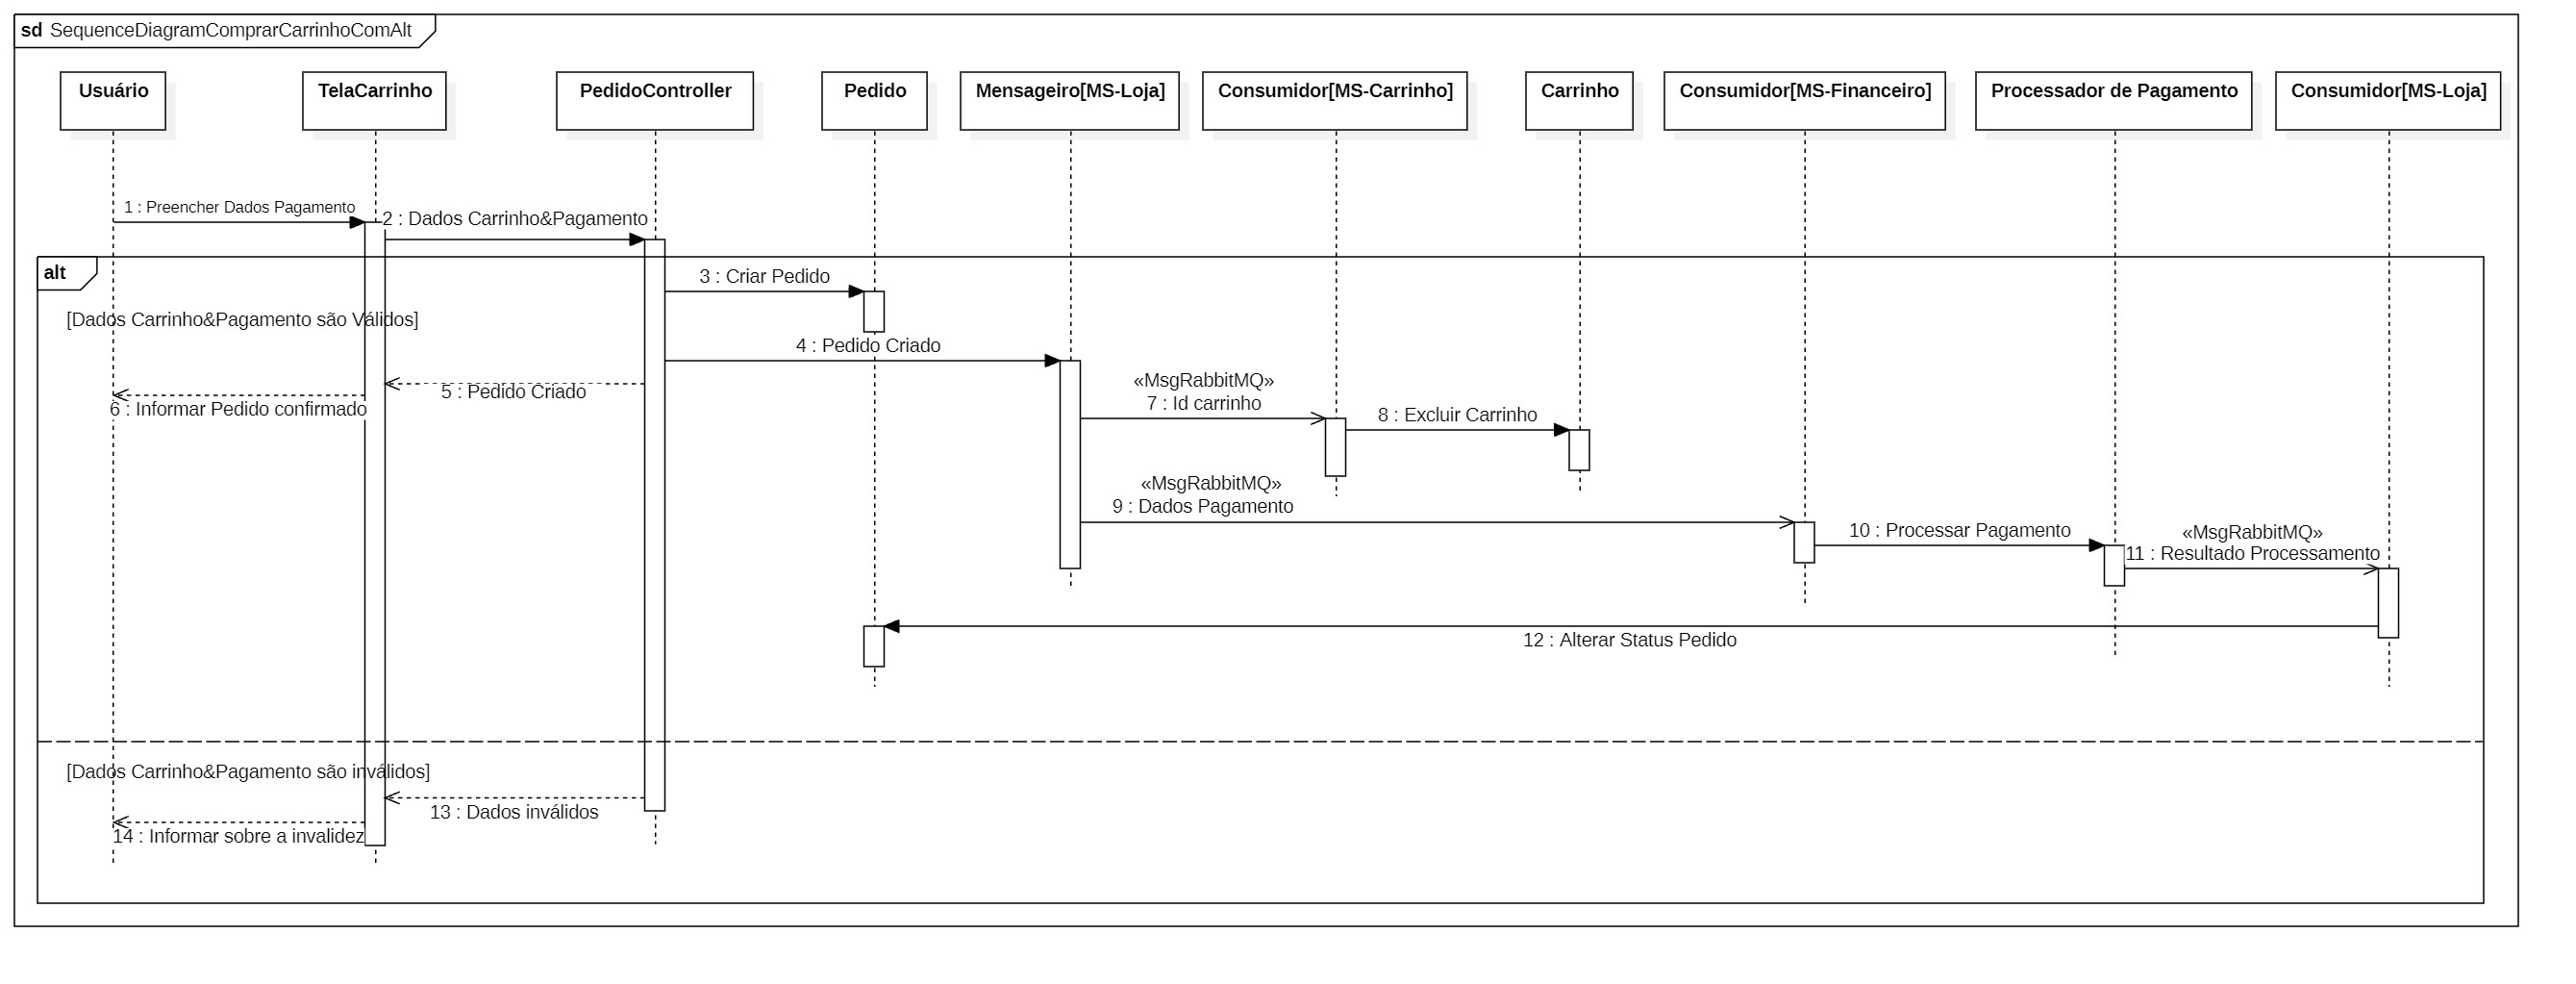
\includegraphics[scale=0.16]{Diagramas/imagens/SequenceComprarCarrinhoComFinanceiroComAlt.jpg}
	\end{center}
	\legend{Fonte: Autor}
\end{figure}


\section{Práticas e ferramentas usadas}
\subsection*{Frameworks e linguagens}
Java+Spring, C\#+.NET, TypeScript+ExpressJS, TypeScript+ReactJS, TypeScript+Angular

\subsection*{Metodologia 12-fatores}
Descrever os fatores cumpridos...

\subsection*{Descentralização dos dados}

\subsection*{CI/CD}
% Mostrar o exemplo do pipeline CI rodando no GitHub Actions, com proteções de branch e requerimento de revisão de código


\subsection*{Organização do código - Multirepo}
Para organização do código foi utilizada a técnica Multirepo, com repositórios no GitHub.

\subsection*{Implantação em contêineres}
Docker e Kubernetes

\subsection*{Testes}
Testes de unidade

\subsection*{Boas práticas em APIs}

\subsection*{Comunicação assíncrona}
RabbitMQ

\subsection*{Monitoramento}
Prometheus, grafana, loki,